\documentclass[12pt,twoside]{article}
\usepackage{amsmath, amssymb}
\usepackage{amsmath}
\usepackage[active]{srcltx}
\usepackage{amssymb}
\usepackage{amscd}
\usepackage{makeidx}
\usepackage{amsthm}
\usepackage{algpseudocode}
\usepackage{algorithm}
\usepackage{graphicx}
\usepackage[spanish]
\renewcommand{\baselinestretch}{1}
\graphicspath{{images/}}
\setcounter{page}{1}
\setlength{\textheight}{21.6cm}
\setlength{\textwidth}{14cm}
\setlength{\oddsidemargin}{1cm}
\setlength{\evensidemargin}{1cm}
\pagestyle{myheadings}
\thispagestyle{empty}
\markboth{\small{Pr\'actica 2. Alan, Josu\'e}}{\small{.}}
\date{}
\begin{document}
\centerline{\bf An\'alisis de Algoritmos, Sem: 2020-1, 3CV2, Pr\'actica 2, 15 de agosto}
\centerline{}
\centerline{}
\begin{center}
\Large{\textsc{Pr\'actica 1: Determinaci\'on experimental de la complejidad temporal de un
algoritmo}}
\end{center}
\centerline{}
\centerline{\bf {Alan Romero Lucero, Josué David Hernández Ramírez}}
\centerline{}
\centerline{Escuela Superior de C\'omputo}
\centerline{Instituto Polit\'ecnico Nacional, M\'exico}
\centerline{$alanrl.escom@gmail.com, correo@alumno_2$}
\newtheorem{Theorem}{\quad Theorem}[section]
\newtheorem{Definition}[Theorem]{\quad Definition}
\newtheorem{Corollary}[Theorem]{\quad Corollary}
\newtheorem{Lemma}[Theorem]{\quad Lemma}
\newtheorem{Example}[Theorem]{\quad Example}
\bigskip
\textbf{Resumen:} En la presente pr\'actica se determino la complejidad temporal, de manera experimental, de los siguientes algoritmos: un algortimo de suma de dos numeros enteros en notaci\'on binaria y el algoritmo de euclides para determinar el \textit{mcd} de dos n\'umeros enteros positivos.
{\bf Palabras Clave:} {\textit{algoritmo, complejidad, iteraciones}}
\section{Introducci\'on}
Los algoritmos son parte de nuestro d\'ia a d\'ia, de forma tal que ni siquiera nos detenemos a pensar en ellos, desde la simple receta de cocina hasta aplicar un m\'etodo matemático para resolver algo. Siguiendo con el ejemplo de un m\'etodo matemático, no es lo mismo, por ejemplo, resolver una integral por partes que por sustituci\'on trigonometric si es que el caso lo permite. Tal vez no es el mejor ejemplo, dado que no son como tal \textit{algoritmos}, sin embargo sirve para percatarse de la importancia de analizar un algoritmo.

Ya entrando en materia, al inicio de la computaci\'on era verdaderamente importante analizar el algoritmo que una computadora ejecutaría dado lo limitadas que se encontraban las computadoras en ese momento; entonces ser\'ia tentador pensar que actualmente no existe esa limitante, no obstante, es muy importante seguir cuidando los tiempos de ejecuci\'on de un algoritmo, hace falta pensar en lo que se puede hacer con la capacidad de las computadoras actuales si se analiza correctamente un algoritmo. El objetivo de esta pr\'actica es ese, analizar dos algoritmos relativamente simples, la suma de números binarios y el algoritmo de Euclides,entender su comportamiento en diversas situaciones as\'i como determinar su complejidad de manera experimental.
\section{Conceptos B\'asicos}
Para entender mejor la pr\'actica hace falta definir lo que es la \textit{notaci\'on theta($\Theta$), big O($O$) y omega($\Omega$)}.
\newline

\textbf{Theta ($\Theta$).} Define limites superiores e inferior a una funci\'on $g(n)$ dada. Definido de la siguiente forma: 
\begin{center}
    $\Theta(g(n))$ = \{ $f(n)$ $|$ $\exists$  $c\textsubscript{1}, c\textsubscript{2}, n\textsubscript{0}$ tal que $0 \leq c\textsubscript{1}g(n)\leq f(n)\leq c\textsubscript{2}g(n)$ $\forall$ $n\geq n\textsubscript{0}$ \}
\end{center}

\textbf{Big O ($O$).} Define el limite superior de una funci\'on $g(n)$ dada. Definido de la siguiente forma: 
\begin{center}
    $O(g(n))$ = \{ $f(n)$ $|$ $\exists$  $c, n\textsubscript{0}$ tal que $0 \leq f(n)\leq cg(n)$ $\forall$ $n\geq n\textsubscript{0}$ \}
\end{center}

\textbf{Omega ($\Omega$).} Define el limite inferior a una funci\'on $g(n)$ dada. Definido de la siguiente forma: 
\begin{center}
    $\Omega(g(n))$ = \{ $f(n)$ $|$ $\exists$  $c, n\textsubscript{0}$ tal que $0 \leq cg(n)\leq f(n)$ $\forall$ $n\geq n\textsubscript{0}$ \}
\end{center}

Para \textbf{el algoritmo de suma binaria} se implementa el siguiente algoritmo:
\begin{algorithmic}
    \Require a, b
    \Ensure k = $\log_{2} (m)$, t = $\log_{2} (n)$, donde n y m es la longitud de a y b
    \State i $\longleftarrow$ k
    \State carry $\longleftarrow$ 0
    \While{$i\geq0$}
        \If {$(a[i]+b[i]+c)=1$}
            \State $c$ \textbf{insertar al inicio} $1$
            \State carry $\longleftarrow$ 0
        \ElsIf {$(a[i]+b[i]+c)=2$}
            \State $c$ \textbf{insertar al inicio} $0$
            \State carry $\longleftarrow$ 1
        \ElsIf {$(a[i]+b[i]+c)=3$}
            \State $c$ \textbf{insertar al inicio} $1$
            \State carry $\longleftarrow$ 1
        \Else
            \State $c$ \textbf{insertar al inicio} $0$
            \State carry $\longleftarrow$ 0
        \EndIf
        \State i $\longleftarrow$ i - 1
    \EndWhile
    \If{$carry = 1$}
        \State carry $\longleftarrow$ 1
    \EndIf
    \State \Return c
    
\end{algorithmic}

El funcionamiento del algoritmo es simple, recorre todo el arreglo y verifica s\'i la suma de los elementos de a y b en i, mas el acarreo. S\'i el resultado de la suma es uno, inserta cero al resultado e inicializa en uno el acarreo; s\'i es dos, inserta cero al resultado y guarda uno en el acarreo; s\'i es tres, inserta uno al resultado y guarda uno en el acarreo; finalmente, de otra forma inserta cero al resultado e inicializa en cero el acarreo. Para terminar, si el acarreo es uno se inserta al resultado

Para \textbf{el algoritmo de Euclides} el pseudo código es el inclu\'ido en la pr\'actica:
\begin{algorithmic}
    \Require m,n
    \While{n $\not= 0$}
        \State r $\longleftarrow$ $m\mod n$
        \State m $\longleftarrow$ $n$
        \State n $\longleftarrow$ $r$
    \EndWhile
    \State \Return m
\end{algorithmic}
 
\section{Experimentaci\'on y Resultados}
\subsection{Suma binaria}
En la primer captura se muestra la implementaci\'on del algoritmo de suma binario, con n\'umeros generados aleatoriamente y su correspondiente gr\'afica. Como lo dice el plantemaiento de la pr\'actica, la longitud de los arreglos m y n debe ser en potencias de dos. Adem\'as la longitud de los arreglos m y n debe ser la misma.
\begin{center}
    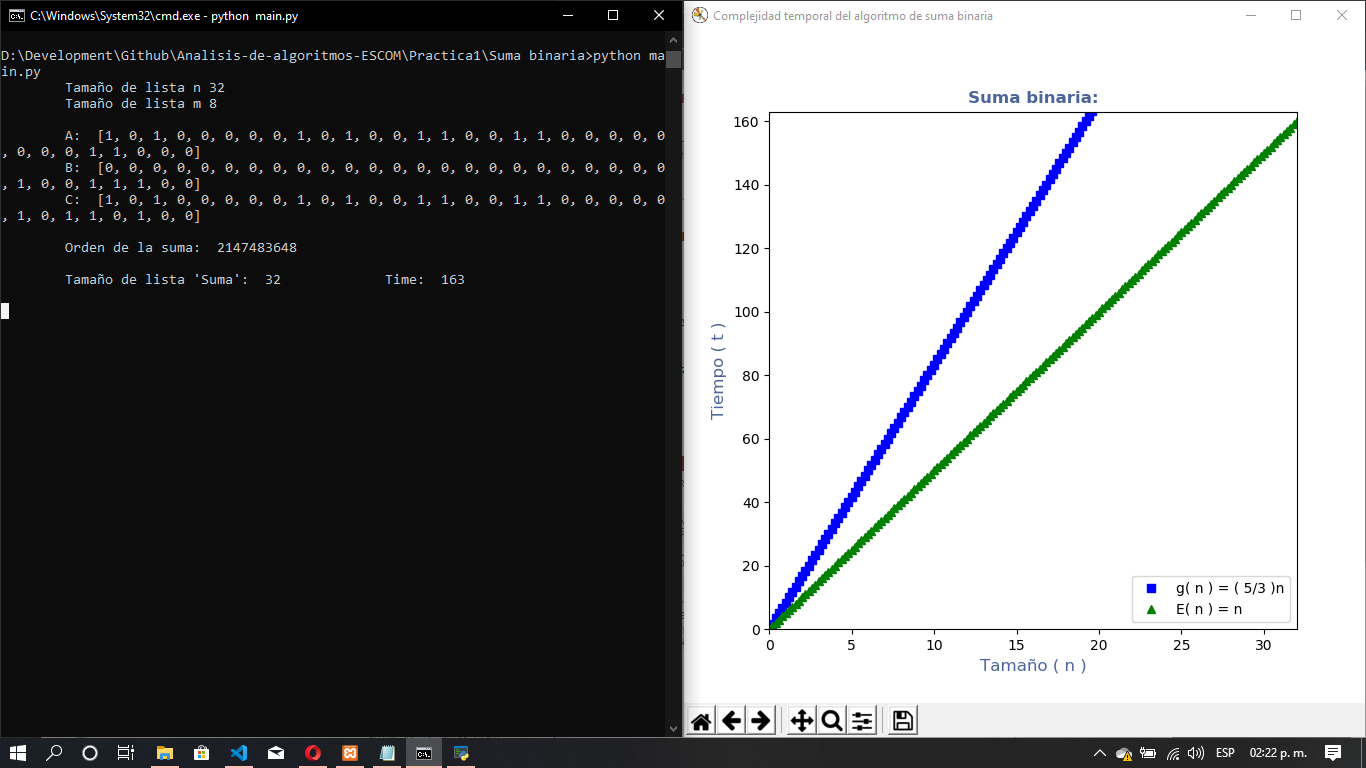
\includegraphics[width = 15cm,height = 8cm ]{68708580_1243798382457972_7674979895071473664_n.png}
\end{center}
En general la funci\'on propuesta para su complejidad, generada de manera experimental, esta marcada con puntos de color azul, $g(n) = 5/3 n$, y su complejidad esta marcada con los puntos de color verde, $E(n) = n$
\begin{center}
    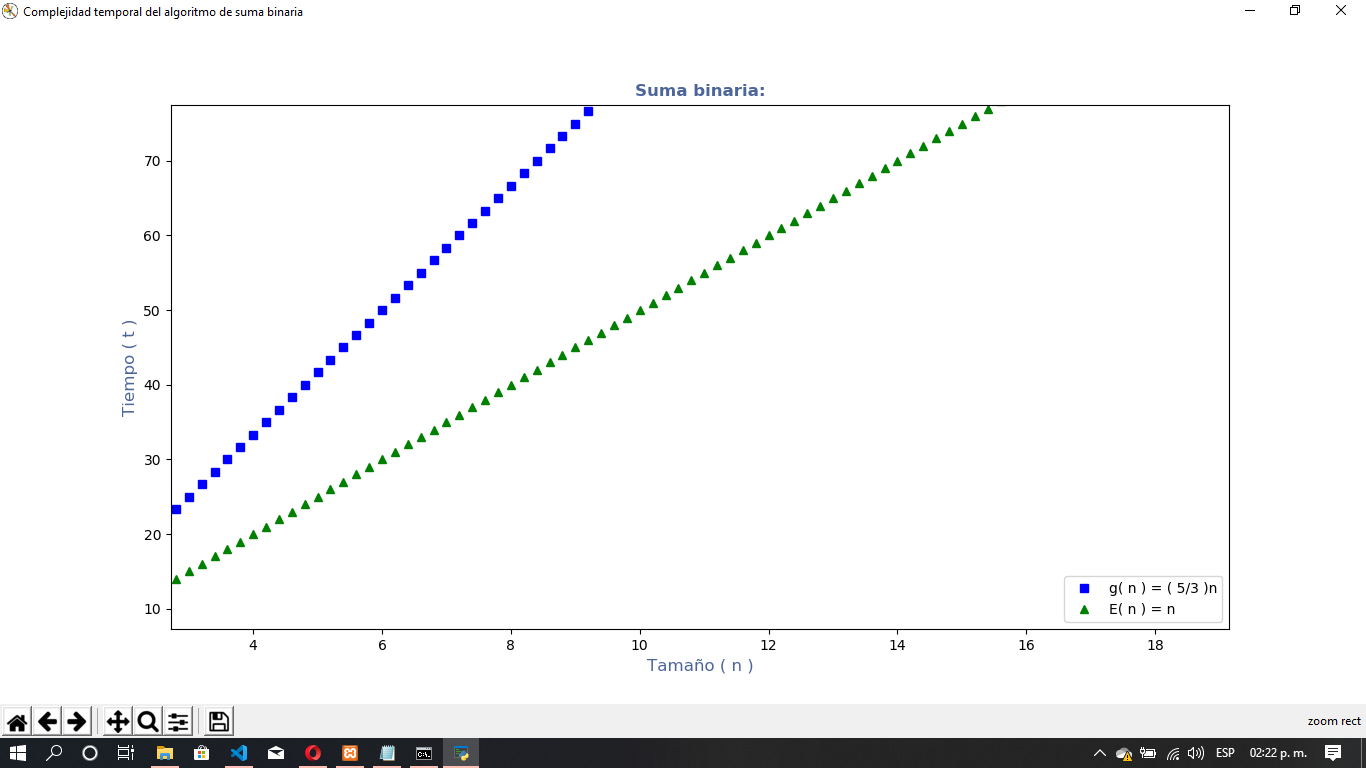
\includegraphics[width = 15cm,height = 8cm ]{69420031_457380968446209_8343133779623149568_n.png}
\end{center}
Es evidente que la complejidad del algoritmo es lineal, tanto por su gr\'afica como por la complejidad ya expresada.
\subsection{Algoritmo de Euclides}
El algoritmo de Euclides podr\'ia resultar mas interesante de analizar, puesto que su complejidad es logarítmica. En su implementaci\'on, primer se experimento con un par de n\'umeros generados de manera aleatoria.
\begin{center}
    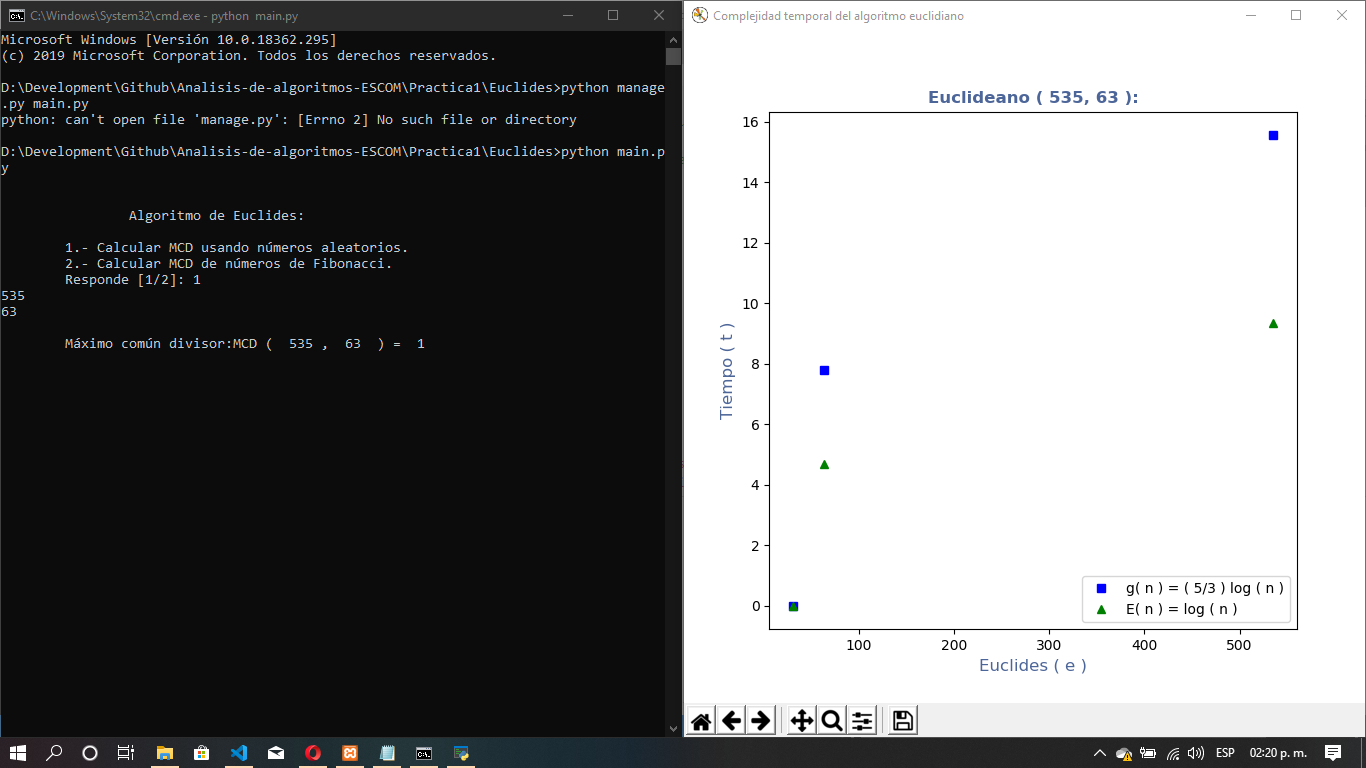
\includegraphics[width = 15cm,height = 8cm ]{69376542_1249778691866556_2742283532700221440_n.png}
\end{center}
Los puntos aparecen relativamente dispersos y no es tan f\'acil visualizar la gr\'afica de su complejidad. Finalmente, utilizando n\'umeros de la sucesi\'on de Fibonacci, dado que representa el peor caso, la gr\'afica se puede ver claramente.
\begin{center}
    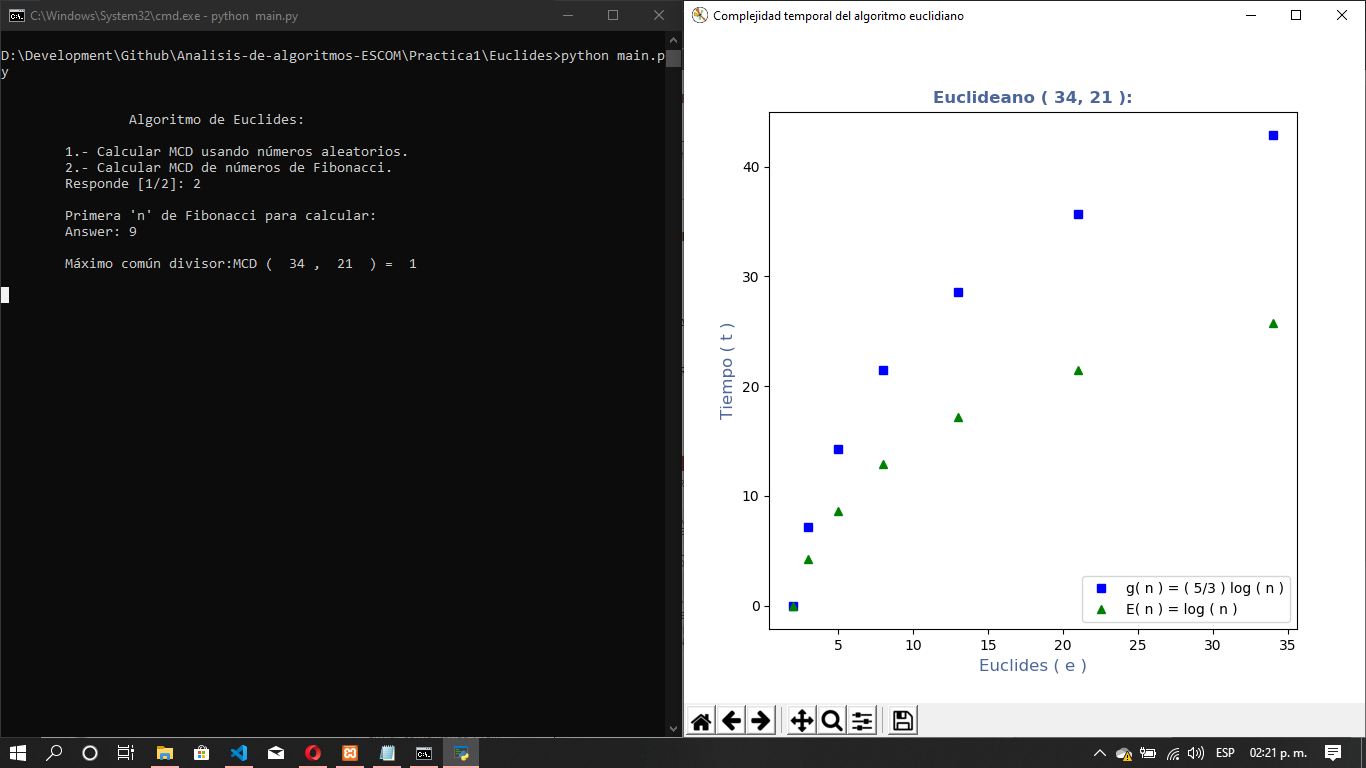
\includegraphics[width = 15cm,height = 8cm ]{69398675_892639287772849_6709061515640569856_n.png}
\end{center}
La funci\'on planteada es $g(n)=5/3\log (n)$, mientras que su complejidad es, efectivamente $E(n) = \log (n)$
\section{Conclusiones}
La implementaci\'on del algoritmo de Euclides resulto en un error interesante, en el que, al generar los datos necesarios para graficar la complejidad del algoritmo estos se generaban invertidos, por lo que los puntos en el plano resultaban incorrectos. La soluci\'on fue simplemente invertir el arreglo con los datos que se usaban para gr\'aficar.

\textit{Alan Romero Lucero}. El algoritmo de suma binaria me parece interesante dada su complejidad ya que, pese a ser lineal, me parece relativamente \textit{"complejo"}, comparado con el de Euclides, por ejemplo, que es logarítmico. Sin embargo, no se me ocurrió una manera de simplificar el algoritmo. Es interesante ver como se comportan los algoritmos.

\textit{Josué David Hernández Ramírez}. El desarrollo de estos algoritmos para poder a empezar a entender el significado de complejidad a los algoritmos fue bastante interesante, puesto que al programarlos y mostrar los resultados expresados mediante el uso de librerías para la graficación se aprecia de manera visual el concepto de complejidad, ya que este esté sujeto al tiempo en que tarda en concretarse el algoritmo, lo cual es lo que comprobamos al realizar esta práctica. Fue un poco tediosa al tener que manejar datos aleatorios y la creación de listas y su manipulación para las operaciones necesarias.

\section{Anexo}
\begin{center}
Se dej\'o como problema a resolver el algoritmo del  \textit{\textbf{select-sort}}.
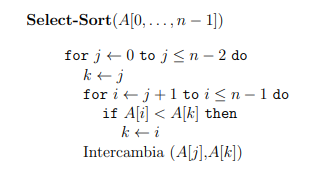
\includegraphics[width = 10cm,height = 6cm ]{anexo.png}
\end{center}
Analizando linea por linea, haciendo el calculo en el peor de los casos, donde estan el arreglo esta invertido.
\begin{center}
\begin{tabular}{ |c|c|c| } 
 \hline
 \textbf{Linea/Constante de tiempo} & \textbf{Conteo} \\ 
 $c1$ & $n-1$ \\ 
 $c2$ & $n-2$ \\  
 $c3$ & $\sum_{i=1}^{n-2} t\textsubscript{i}$ \\
 $c4$ & $\sum_{i=1}^{n-2} (t\textsubscript{i} - 1)$ \\
 $c5$ & $\sum_{i=1}^{n-1} (t\textsubscript{i} - 1)$ \\ 
 $c6$ & $k$ \\ 
 \hline
\end{tabular}
\end{center}
Entonces, por cada linea se tiene:
\newline
\begin{itemize}
    \item $(c\textsubscript{1})(n-1)$
    \item $(c\textsubscript{2})(n-2)$
    \item $(c\textsubscript{3})(\sum_{i=1}^{n-2} t\textsubscript{i})$
    \item $(c\textsubscript{4})(\sum_{i=1}^{n-2} (t\textsubscript{i} - 1))$
    \item $(c\textsubscript{5})(\sum_{i=1}^{n-1} (t\textsubscript{i} - 1))$
    \item $(c\textsubscript{6})(k)$
\end{itemize}
Finalmente, simplificando todo, se llega a una expresión $g(n)=an\textsuperscript{2}+bn+c$, por lo que $g(n)\in O(n\textsuperscript{2})$
\section{Bibliograf\'ia}
"Notación O mayúscula", class notes for Análisis de Algoritmos, ESCOM-IPN, Verano 2019.
\end{document}
